\section{Livello 2: Data Link}
    \subsection{Scopo e panoramica del livello}
        Il livello \textit{data link} ha la responsabilità di trasferire in modo sufficientemente affidabile i dati tra nodi adiacenti, ovvero su canali punto-punto o multi-accesso.

        La comunicazione affidabile è realizzata mediante le seguenti funzionalità: il flusso di dati viene suddiviso in \textbf{frame} con lunghezza massima fissata. Il \textit{frame} contiene un \textbf{payload} che viene riempito con i dati da trasportare provenienti dal livello superiore e informazioni di servizio poste in testa e/o in coda al payload (\textbf{header/trailer}).

        Per ogni frame deve essere applicato un meccanismo per la rilevazione ed eventualmente la correzione degli errori. Il livello deve poter gestire il controllo del flusso Nei canali multi-accesso deve occuparsi anche dell'accesso al mezzo trasmissivo.
        
        I servizi offerti al livello network possono essere:
        \begin{itemize}
            \item \textbf{Senza connessione e senza conferma}: e semplice e veloce, è adatto a mezzi trasmissivi affidabili (es. LAN Wired).
            \item \textbf{Senza connessione ma con conferma}: viene inviato un frame di conferma per ogni frame inviato, è utili se il mezzo trasmissivo è poco affidabile (es. LAN Wireless).
            \item \textbf{Con connessione e con conferma}: ogni frame inviato è parte di una connessione, e quindi è dotato di una numerazione; offre la garanzia che ogni frame inviato viene ricevuto una sola volta ed ordinato, ha un overhead elevato, viene utilizzato raramente nel livello data link. Comprende tre fasi disinte:
            \begin{itemize}
                \item Attivazione di una connessione.
                \item Invio dei dati numerati con relativa conferma.
                \item Chiusura della connessione.
            \end{itemize}
        \end{itemize}

    \subsection{Framing}
        Il problema da risolvere è come delimitare inizio e termine di un frame.
    
        I frame possono avere dimensione fissa o variabile. Se la dimensione è fissa non è necessario delimitare il frame (vedi la rete ATM). Se la dimensione è variabile occorre una strategia per distinguere i frame.
    
        Un intervallo temporale tra un frame ed il successivo non è una garanzia sufficiente di delimitazione. Metodi più attendibili sono:
        \begin{itemize}
            \item Far precedere ogni frame con il numero di byte del frame.
            \item Delimitare il frame con caratteri speciali (flag).
        \end{itemize}

        Gran parte dei protocolli di data link usano l'abbinamento del flag e dell'intervallo temporale per aumentare la ridondanza.

        \subsubsection{Framing con conteggio dei byte}
            Il numero dei byte viene scritto nell'intestazione.

            È poco utilizzato poiché un errore di trasmissione del contatore potrebbe mettere fuori sincronismo i frame successivi.

            \begin{center}
    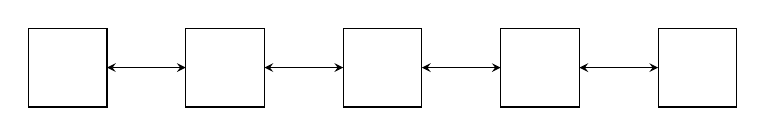
\begin{tikzpicture}
        %%%%%%%%%% Nodi %%%%%%%%%%
        \foreach \x in {0,2,...,8}
            \draw (\x,0) rectangle ++(1,1);

        %%%%%%%%% Frecce %%%%%%%%%
        \foreach \x in {1,3,...,7}
            \draw[<->,>=stealth] (\x,0.5) -- ++(1,0);
    \end{tikzpicture}
\end{center}

        \subsubsection{Framing con ESC stuffing}
            La delimitazione del frame è marcata da un byte speciale denominato \textbf{FLAG}.

            Un problema potrebbe nascere se all'interno del frame è presente la sequenza di FLAG.

            Per flussi \textbf{byte-oriented}, si può inserire un byte di Escape (\textbf{ESC}) appena prima dell'occorrenza accidentale di FLAG o di ESC).

            \begin{center}
    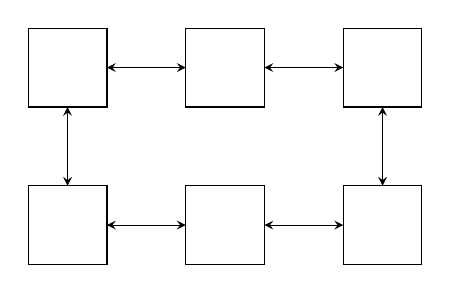
\begin{tikzpicture}
        %%%%%%%%%% Nodi %%%%%%%%%%
        \draw (0,0) rectangle (1,1);
        \draw (2,0) rectangle (3,1);
        \draw (4,0) rectangle (5,1);
        \draw (0,2) rectangle (1,3);
        \draw (2,2) rectangle (3,3);
        \draw (4,2) rectangle (5,3);

        %%%%%%%%% Frecce %%%%%%%%%
        \draw[<->,>=stealth] (1,0.5) -- (2,0.5);
        \draw[<->,>=stealth] (3,0.5) -- (4,0.5);
        \draw[<->,>=stealth] (1,2.5) -- (2,2.5);
        \draw[<->,>=stealth] (3,2.5) -- (4,2.5);
        \draw[<->,>=stealth] (0.5,1) -- (0.5,2);
        \draw[<->,>=stealth] (4.5,1) -- (4.5,2);
    \end{tikzpicture}
\end{center}

            Il destinatario dovrà realizzare l'operazione di destuffing.

        \subsubsection{Bit stuffing}
            Se i flussi sono \textbf{bit-oriented} si può utilizzare il bit-stuffing: ogni frame inizia e termina con la sequenza \textbf{01111110} (FLAG).

            Ogni volta che nella trama si incontra la sequenza 11111 (5 uni) viene aggiunto un bit 0 (bit stuffing) per non confondere i destinatari. Viene utilizzato in HDLC.
            
            \subsubsection*{Procedimento:}
            \begin{enumerate}[label=(\alph*)]
                \item \texttt{011011111111111111110010}
                \item \texttt{011011111\underline{0}11111\underline{0}11111\underline{0}10010}
                \item \texttt{011011111111111111110010}
            \end{enumerate}

            \subsubsection*{Legenda:}
            \begin{enumerate}[label=(\alph*)]
                \item Dati originali
                \item Dati elaborati dal mittente che aggiunge i bit di stuffing
                \item Dati elaborati dal destinatario che elimina i bit di stuffing
            \end{enumerate}

    \subsection{Rilevazione e correzione degli errori}
        Durante la trasmissione di un frame possono verificarsi disturbi o rumore termico che possono cambiare la forma del segnale e quindi alterare la ricezione dei bit.

        Tipi di errori sono:
        \begin{itemize}
            \item a bit singolo
            \item a raffica (burst)
        \end{itemize}

        Per individuare gli errori si utilizza la ridondanza: il mittente, attraverso un opportuno algoritmo, determina una breve codice \textbf{FCS (Frame Control Sequence)}, che verrà inviato assieme al frame.
        
        Se il destinatario riapplicando l'algoritmo otterrà una sequenza FCS diversa capirà che si è verificato un errore.

        Esistono due strategie disponibili:
        \begin{itemize}
            \item \textbf{Rilevazione degli errori}: richiede algoritmi più semplici ed un FCS più breve. Si utilizza su canali affidabili (es. fibra ottica), in cui gli errori sono rari e conviene eventualmente ritrasmettere il frame. La richiesta di ritrasmissione può essere esplicita (il ricevente manda un NACK in caso di errore) o automatica con protocollo ARQ (il mittente attiva un timer, il ricevente invia un ACK per i dati ricevuti correttamente e scarta i dati con errore, allo scadere del timer il mittente rispedisce il frame).
            \item Rilevazione e correzzione degli errori: richiede algoritmi più complessi e maggiore ridondanza nel FCS. Si utilizza in reti poco affidabili (es. WiFi) o, in trasmissioni simplex, in cui non è possibile inviare al mittente la richiesta di ritrasmissione.
        \end{itemize}

        \subsubsection{Codifica a blocchi: bit di parità}
            Semplice algoritmo esemplificativo per rilevazione e correzione dell'errore.
        
            Il numero totale di 1 nella sequenza, compreso il bit di parità, deve essere dispari (o pari).

            Applicato alla sequenza di un frame determina l'esistenza di un singolo errore. Suddividendo il frame in più sotto-sequenze di uguale lunghezza possiamo calcolare la parità in due dimensioni e quindi individuare e correggere il singolo bit errato.
            
            Il bit di parità si usa in molti dispositivi hardware come ad esempio nei bus SCSI e USB e in molte cache di microprocessori.

            \begin{center}
    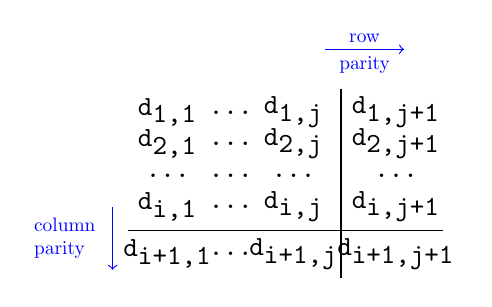
\begin{tikzpicture}
        %%%%%%%%% Testo %%%%%%%%%%
        \node at (1,5.2) {\texttt{d$_{\texttt{1,1}}$}};
        \node at (1.8,5.2) {\texttt{...}};
        \node at (2.6,5.2) {\texttt{d$_{\texttt{1,j}}$}};
        \node at (1,4.8) {\texttt{d$_{\texttt{2,1}}$}};
        \node at (1.8,4.8) {\texttt{...}};
        \node at (2.6,4.8) {\texttt{d$_{\texttt{2,j}}$}};
        \node at (1,4.4) {\texttt{...}};
        \node at (1.8,4.4) {\texttt{...}};
        \node at (2.6,4.4) {\texttt{...}};
        \node at (1,4) {\texttt{d$_{\texttt{i,1}}$}};
        \node at (1.8,4) {\texttt{...}};
        \node at (2.6,4) {\texttt{d$_{\texttt{i,j}}$}};
        \node at (1,3.4) {\texttt{d$_{\texttt{i+1,1}}$}};
        \node at (1.8,3.4) {\texttt{...}};
        \node at (2.6,3.4) {\texttt{d$_{\texttt{i+1,j}}$}};

        \node at (3.9,5.2) {\texttt{d$_{\texttt{1,j+1}}$}};
        \node at (3.9,4.8) {\texttt{d$_{\texttt{2,j+1}}$}};
        \node at (3.9,4.4) {\texttt{...}};
        \node at (3.9,4) {\texttt{d$_{\texttt{i,j+1}}$}};
        \node at (3.9,3.4) {\texttt{d$_{\texttt{i+1,j+1}}$}};

        %%%%%%%%%% Assi %%%%%%%%%%
        \draw (0.5,3.7) -- (4.5,3.7);
        \draw (3.2,3.1) -- (3.2,5.5);

        %%%%%%%%% Frecce %%%%%%%%%
        \draw[->,blue] (3,6) -- node[above,scale=0.7] {row} node[below,scale=0.7]{parity} (4,6);
        \draw[->,blue] (0.3,4) -- node[left,scale=0.7,text width=1.3cm] {column parity} (0.3,3.2);
    \end{tikzpicture}
\end{center}
            \vbox{}
            \begin{center}
    \begin{tikzpicture}
        %%%%%%%%%% Nodi %%%%%%%%%%
        \draw (0,0) rectangle (1,1);
        \draw (2,0) rectangle (3,1);
        \draw (4,0) rectangle (5,1);
        \draw (6,0) rectangle (7,1);
        \draw (8,0) rectangle (9,1);
        \draw (10,0) rectangle (11,1);
        \draw (2,2) rectangle (3,3);
        \draw (8,2) rectangle (9,3);
        \draw (5,4) rectangle (6,5);

        %%%%%%%%% Frecce %%%%%%%%%
        \draw[<->,>=stealth] (0.5,1) -- (2,2);
        \draw[<->,>=stealth] (2.5,1) -- (2.5,2);
        \draw[<->,>=stealth] (4.5,1) -- (3,2);
        \draw[<->,>=stealth] (6.5,1) -- (8,2);
        \draw[<->,>=stealth] (8.5,1) -- (8.5,2);
        \draw[<->,>=stealth] (10.5,1) -- (9,2);
        \draw[<->,>=stealth] (2.5,3) -- (5,4);
        \draw[<->,>=stealth] (8.5,3) -- (6,4);
    \end{tikzpicture}
\end{center}

            Le frecce rosse indicano la presenza di un \textit{parity error}.

        \subsubsection{Cyclic Redundancy Check (CRC)}
            Un Frame di $d$ bit è visto come una lista di coefficienti di un polinomio $D$ con $d$ termini (di grado $d-1$). Per esempio 110001 rappresenta $x^5 + x^4 + x^0$.

            Trasmettitore e ricevitore si mettono d'accordo su di un polinomio comune $G$ di $r + 1$ bit (grado $r$) detto generatore, che deve essere un numero primo.

            Il Trasmettitore aggiunge $r$ bit (il CRC) al termine della sequenza del frame in modo che il nuovo frame $M$ (di grado $r+d-1$) sia divisibile per $G$.

            Procedura:
            \begin{enumerate}
                \item $N = D \cdot x^r$ (vengono aggiunti $r$ zeri al termine di $D$)
                \item $R = \frac{N}{G}$ (viene determinato il resto $R$ della divisione)
                \item $M = N - R = N \oplus R$ ($N-R$ è divisibile per $G$. La sottrazione in $mod_2$ si fa con XOR).
            \end{enumerate}

            Il ricevitore divide $M/G$. Se il resto è diverso da zero si è verificato un errore.

            Procedura:
            \begin{enumerate}
                \item $R = \frac{M}{G}$ (viene determinato il resto $R$ della divisione)
                \item Se $R \neq 0$ allora si è verificato un errore.
            \end{enumerate}

            \begin{center}
                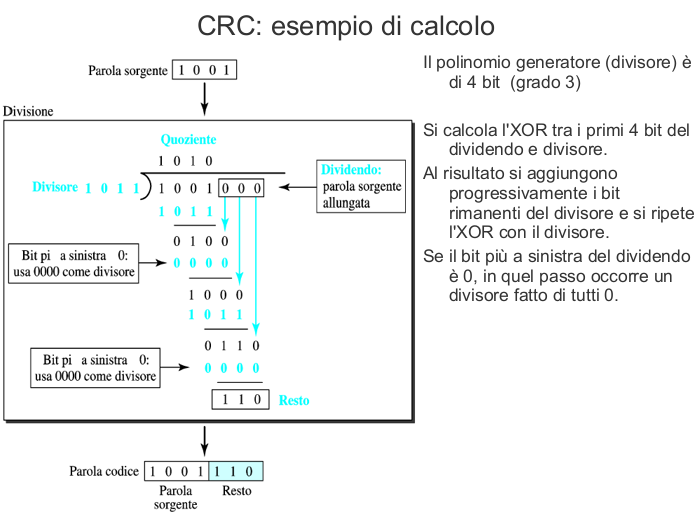
\includegraphics[scale=0.4]{chapters/3/assets/schema_e.png}
            \end{center}

            Uno dei vantaggi del CRC è che i moduli di codifica e decodifica possono essere facilmente implementati in hardware usando componenti elettronici poco costosi.

            La codifica polinomiale CRC con $r$ bit di controllo è in grado di rilevare sequenze di errori di lunghezza fino a $r$.

            Il CRC è il codice più utilizzato nei protocolli data link:
            \begin{itemize}
                \item Ethernet: usa il CRC-32 ($x^{32} +x^{26} +x^{23} +x^{22} +x^{16} +x^{12} +x^{11} +x^{10} +x^8 + x^7 +x^5 +x^4 +x^2 +x^1 +x^0$) riesce a rilevare fino a 32 errori e tutti quelli che toccano un numero dispari di bit.
                \item HDLC: usa il CRC-16.
                \item ATM: usa il CRC-8.
            \end{itemize}

        \subsubsection{Checksum (somme di controllo)}
            Si sommano in complemento ad 1 su 16 bit tutti i dati del messaggio. Il checksum (16 bit) è il complemento del risultato.

            \newpage
            \lstinputlisting{chapters/3/assets/schema_f.c}

            È molto adatto per implementazioni software e per questo è usato nei protocolli di Internet (IP, ICMP, TCP, UDP, etc.).

    \subsection{Protocolli di comunicazione per canali senza rumore}
        \subsubsection{Protocollo simplex}
            Questo protocollo si affida su uno scenario ideale (utopistico):
            \begin{itemize}
                \item Il destinatario è sempre pronto a ricevere ed a gestire i frame ricevuti.
                \item I dati arrivano senza errori.
            \end{itemize}

            \begin{center}
                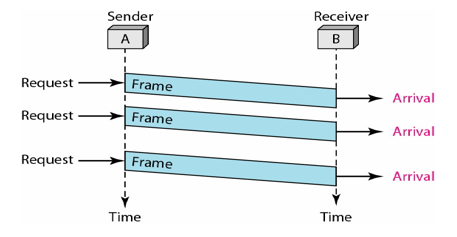
\includegraphics[scale=0.6]{chapters/3/assets/schema_g.png}
            \end{center}

        \subsubsection{Protocollo stop-and-wait}
            Lo scenario è il seguente:
            \begin{itemize}
                \item Il ricevente ha bisogno di tempo per elaborare i dati ricevuti.
                \item I dati arrivano senza errori.
            \end{itemize}

            Prima di inviare il prossimo dato, il mittente deve ricevere una conferma \textbf{ACK}, per cui il destinatario, se sovraccarico, può moderare il tasso di invio dei dati ritardando l'invio dell'ACK.

            \begin{center}
                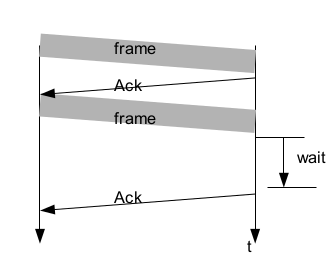
\includegraphics[scale=0.6]{chapters/3/assets/schema_h.png}
            \end{center}

    \subsection{Protocollo per canali con rumore}
        \subsubsection{Protocollo stop-and-wait ARQ}
            Lo scenario è il seguente:
            \begin{itemize}
                \item Il ricevente ha bisogno di tempo per elaborare i dati ricevuti.
                \item I frame possono essere danneggiati o perduti.
            \end{itemize}

            Poiché i Frame possono andare perduti, viene gestita una numerazione dei Frame e dei relativi ACK. I frame danneggiati vengono scartati, oppure viene inviato un \textbf{NACK} (Not ACK).

            Per gestire la perdita dei frame, il mittente attiva un timer per ogni frame inviato; se il mittente non riceve un ACK in un determinato periodo di tempo, il frame viene rispedito.
            
            Il protocollo offre un servizio di connessione con consegna garantita ed ordinata grazie alla numerazione ed al rinvio.

            Il mittente deve mantenere copia dei frame fino all'ACK.

            Se il traffico è bidirezionale, l'ACK può viaggiare in un frame inviato in senso opposto (\textbf{piggybacking}).

            Nei protocolli stop-and-wait la capacità del canale non è efficiente.

            \begin{center}
                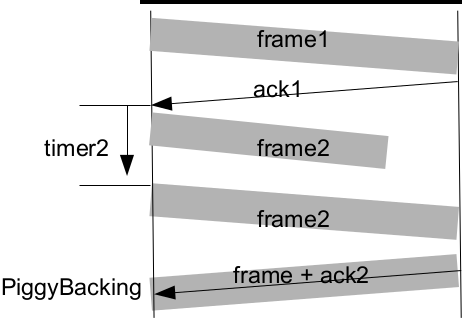
\includegraphics[scale=0.45]{chapters/3/assets/schema_i.png}
            \end{center}

        \subsubsection{Protocollo Sliding Window}
            I protocolli di tipo \textit{Sliding Window} migliorano l'efficienza del canale consentendo al trasmettitore di poter inviare fino ad $N$ frame senza riscontro.
        
            $N$ rappresenta la dimensione della finestra dei frame senza riscontro, che si sposta in avanti man mano che i riscontri arrivano. I frame appartenenti alla finestra vengono memorizzati dal mittente per eventuali ritrasmissioni.

            Il mittente assegna ad ogni frame un \textit{numero di sequenza}.

            L'indice \textbf{LFS (Last Frame Sent)} contiene il numero dell'utimo frame inviato, l'indice \textbf{LAR (Last Ack Received)} contiene l'indice dell'ultimo ACK ricevuto, la \textbf{SWS (Send Window Size)} è dimensione della finestra del trasmettitore e deve valere che:

            \begin{equation*}
                LFS - LAR \leq SWS
            \end{equation*}

            La finestra del destinatario specifica i frame che il destinatario può ricevere in quel momento. In genere corrisponde allo spazio libero nel buffer del ricevente.

            La finestra del mittente specifica i frame che il mittente può spedire in quel momento non può superare la finestra del destinatario (può essere ridotta per altri motivi).

            \begin{center}
                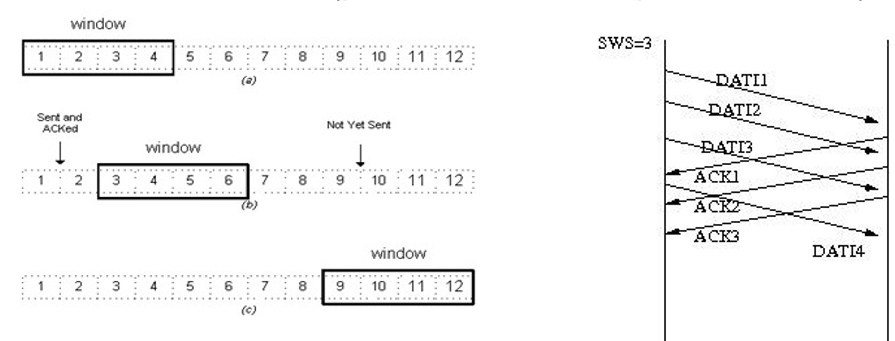
\includegraphics[scale=0.38]{chapters/3/assets/schema_j.png}
            \end{center}

        \subsubsection{Protocollo Go-Back-N ARQ}
            Con il protocollo \textit{sliding window} può succedere che un frame risulti errato (o vada perduto) quando diversi altri frame successivi sono già stati inviati.
        
            Se al destinatario arrivano frame fuori ordine (successivi a frame non ancora riscontrati) li scarta. Solo i Frame arrivati correttamente (senza errori e in ordine) vengono mantenuti nel buffer del destinatario fino a quando l'applicazione non li gestisce.
        
            Quando scade il timer del frame errato/perduto il mittente torna indietro e ricomincia a spedire tutti i frame a partire da quello errato (Go-Back-N).

            Il protocollo stop-and-wait ARQ è un caso speciale del protocollo Go-back-N ARQ, in cui la grandezza della finestra è 1.

        \subsubsection{Ripetizione selettiva ARQ}
            Con il protocollo a ripetizione selettiva, i pacchetti successivi a quello errato o perduto vengono bufferizzati dal ricevente, il quale invia un eventuale NACK:
            \begin{itemize}
                \item Il mittente spedisce solo il frame errato (NACK ricevuto) o perduto (time-out).
                \item Il ricevente riscontra il frame errato e tutti i successivi.
            \end{itemize}

            Il destinatario deve mantenere copia in un buffer dei frame ricevuti fuori ordine.

            \begin{center}
                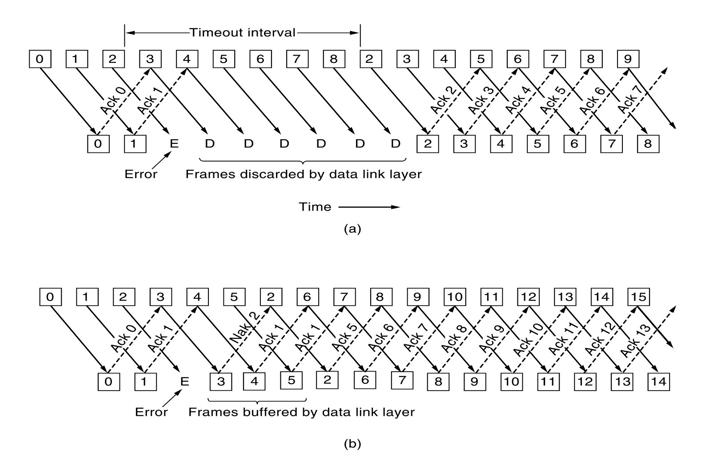
\includegraphics[scale=0.48]{chapters/3/assets/schema_k.png}
            \end{center}

    \subsection{Protocollo PPP}
        È un protocollo byte-oriented (byte stuffing), il quale definisce delle procedure di autenticazione. Supporta vari protocolli dello strato rete (IP, AppleTalk, etc.), fornisce la configurazione degli indirizzi di rete (IP via DHCP), non supporta la modalità non connessa.

        I Frame PPP aggiunge un'intestazione di 6 (o 8) byte al payload, in cui vengono definiti alcuni campi (ideati per HDLC).

        \begin{center}
    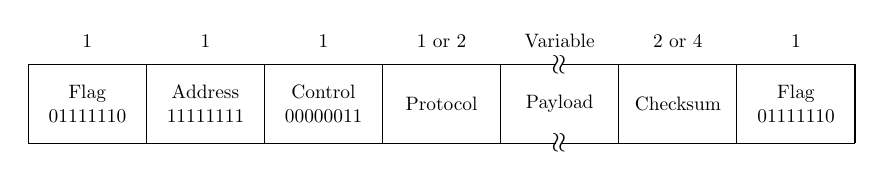
\begin{tikzpicture}
        %%%%%%%% Blocchi %%%%%%%%%
        \draw (0,0) -- ++(6.7,0) ++ (.08,0) -- (10.5,0);
        \draw (0,1) -- ++(6.7,0) ++ (.08,0) -- (10.5,1);
        \node[rotate=90] at (6.75,0) {$\approx$};
        \node[rotate=90] at (6.75,1) {$\approx$};

        \foreach \x in {0,1.5,...,10.5}
            \draw (\x,0) -- ++(0,1);

        %%%%%%%%% Testo %%%%%%%%%%
        \node[align=center,text width=1.4cm,scale=0.7] at (0.75,0.5) {Flag 01111110};
        \node[align=center,text width=1.4cm,scale=0.7] at (2.25,0.5) {Address 11111111};
        \node[align=center,text width=1.4cm,scale=0.7] at (3.75,0.5) {Control 00000011};
        \node[align=center,text width=1.4cm,scale=0.7] at (5.25,0.5) {Protocol};
        \node[align=center,text width=1.4cm,scale=0.7] at (6.75,0.5) {Payload};
        \node[align=center,text width=1.56cm,scale=0.7] at (8.25,0.5) {Checksum};
        \node[align=center,text width=1.4cm,scale=0.7] at (9.75,0.5) {Flag 01111110};

        \foreach \x in {0.75,2.25,3.75,9.75}
            \node[scale=0.7] at (\x,1.3) {1};

        \node[scale=0.7] at (5.25,1.3) {1 or 2};
        \node[scale=0.7] at (6.75,1.3) {Variable};
        \node[scale=0.7] at (8.25,1.3) {2 or 4};

    \end{tikzpicture}
\end{center}

        Campi dell'header PPP:
        \begin{itemize}
            \item Address e Protocol: derivano da HDLC ed in PPP hanno un valore fisso.
            \item Protocol: è stato aggiunto per supportare protocolli di rete (IP, AppleTalk) o protocolli ausiliari (LCP e NCP).
            \item Payload: contiene un numero variaibile di byte, l'MTU è 296 byte.
            \item FCS: CRC-16, negoziabile fino a CRC-32, in caso di errori il pacchetto viene scartato senza notifica, in caso di errori successivi viene abbattuta la connessione.
        \end{itemize}

    \subsection{Reti a circuito virtuale: ATM}
        \textbf{ATM (Asyncronous Transfer Mode)} è un tecnologia, sviluppata a partire dai primi anni '90, che realizza un'infrastruttura di rete per trasmissione dati, basata su un progetto appartenente al mondo della telefonia.
    
        Lo scopo era quello di fornire una nuova tecnologia ad alte prestazioni che riunisca in unica rete la commutazione di pacchetto e quella di circuito.

        Poich é nasce nel mondo della fonia, i principi base dell’architettura sono adattati a questo tipo di esigenza:
        \begin{itemize}
            \item Commutazione di pacchetto a circuito virtuale.
            \item Qualità del servizio (le trasmissioni telefoniche vengono integrate in quelle dati, ma hanno diversi requisiti di qualità).
            \item Pacchetti (celle) di lunghezza fissa di 53 byte, di cui 5 di intestazione e 48 di payload.
        \end{itemize}

        ATM non ha avuto successo al di fuori delle reti telefoniche, se non per la realizzazione di reti WAN, viceversa la fonia sta diventando sempre più un'applicazione di internet (VoIP).

        \subsubsection{Reti LAN - Local Area Network}
            Un canale multi-accesso (broadcast) è un canale condiviso per l’accesso diretto tra più terminali. Consente di realizzare una rete di calcolatori a livello data link (LAN).
        
            È necessario realizzare uno strato aggiuntivo, detto \textbf{MAC (Medium Access Control)} per disciplinare l'accesso al canale.

            Il canale può essere assegnato agli utenti in modo statico o dinamico.

            Con l'allocazione statica, realizzata con tecniche FDM o TDM, si ha uno spreco di banda se il numero di utenti è inferiore al numero dei canali, viceversa, se il numero di utenti è maggiore del numero dei canali, alcuni non possono comunicare, quindi questa tecnica è estremamente inefficiente.

            L'assegnazione del canale nelle reti LAN è dinamica.

            Un singolo canale viene condiviso da $N$ stazioni, ma viene utilizzato solo da chi deve effettivamente inviare un Frame (assegnazione dinamica).

            Nessuna stazione gestisce il canale, ma tutte le stazioni lo devono contendere, si possono verificare collisioni: l'accesso random implica che un frame potrebbe entrare in collisione con un altro. In questo caso entrambi i frame dovranno essere inviati nuovamente.

            Ci sono due modalità di tempo di trasmissione:
            \begin{itemize}
                \item \textbf{Tempo continuo}: la trasmissione può iniziare in qualunque istante.
                \item \textbf{Slotted}: il tempo è diviso in intervalli detti \textit{slot}. La trasmissione deve coincidere con l'inizio di un intervallo.
            \end{itemize}

            Le stazioni possono, in alcuni casi, verificare lo stato del canale \textbf{CS (Carrier Sense)} prima di decidere se iniziare la trasmissione.

            Il protocollo che gestisce i tempi di trasmissione e le eventuali collisioni è detto \textbf{MA (Multiple Access)}.

    \subsection{Protocolli ad accesso multiplo}
        \subsubsection{ALOHA puro}
            Ogni terminale invia i frame senza accordo con gli altri, l'assenza di conferma viene considerata una collisione con gli altri trasmettitori per cui il frame viene ritrasmesso dopo un intervallo di tempo casuale (\textbf{tempo di backoff}).

            Sia $T$ il \textbf{Frame Time}, ovvero il tempo necessario per trasmettere un frame. I frame hanno lunghezza costante di $L$ bit, quindi:

            \begin{equation*}
                T = \frac{L}{bitrate}
            \end{equation*}

            Il tempo di vulnerabilità, cioè l'intervallo di tempo in cui si può avere una collisione (anche con un singolo bit di entrambi i frame), è $2T$.

            Con $N$ frame generati mediamente nel tempo $T$:
            \begin{itemize}
                \item Se $0 < N < 1$ ci aspettiamo un throughput ragionevole.
                \item Se $N > 1$ si va rapidamente alla paralisi.
            \end{itemize}

            Sia $G$ il numero di frame spediti mediamente durante il tempo $T$, allora:

            \begin{equation*}
                G = N + Frame ~ rispediti
            \end{equation*}

            In un algortimo ottimale $G \rightarrow N$

            Qualunque sia il carico $G$ che si presenta, la capacità di trasporto $S$ (Throughput) è $G$ volte la probabilità $P$ (tramissioni con successo nel tempo di vulnerabilità) ovvero:

            \begin{equation*}
                S = G \cdot P_0
            \end{equation*}

            La probabilità che $K$ frame siano generati mediamente durante il tempo $T$ è data dalla distribuzione di Poisson:

            \begin{equation*}
                P[K] = \frac{G^K \cdot e^{-G}}{K!}
            \end{equation*}

            Per un periodo di vulnerabilità pari a $2T$ la probabilità che nessun altro frame venga generato durante il periodo di vulnerabilità è:

            \begin{equation*}
                P[0] = \frac{G^0 \cdot e^{-2G}}{0!} = e^{-2G}
            \end{equation*}

            Quindi il throughput è:

            \begin{equation*}
                S = G \cdot e^{-G}
            \end{equation*}

        \subsubsection{Slotted ALOHA}
            Consente di aumentare la capacità del canale. Il tempo viene diviso in intervalli discreti, le trasmissioni possono iniziare solo all'inizio di un intervallo.

            Una speciale stazione emette un segnale all'inizio di ogni intervallo per sincronizzare trasmettitori.

            Il tempo di vulnerabilità è $T$ (dimezzato rispetto a Pure ALOHA):

            \begin{equation*}
                S = G \cdot e^{-G}
            \end{equation*}

        \subsubsection{Algoritmo di backoff}
            In caso di collisione, parte un algoritmo (detto algoritmo di \textit{backoff}) che determina un tempo di attesa prima di riprovare.

            L'algoritmo di backoff più utilizzato (Ethernet) è l'\textbf{esponenziale binario}: dopo $n$ collisioni consecutive si attende un numero di slot random $x$:

            \begin{equation*}
                0 \leq x \leq 2n - 1
            \end{equation*}

            Dopo una collisione si sceglie tra 0 (riprova subito) e 1 (attendi uno slot). Ethernet ammette un valore massimo di $n$ = 10.

        \subsubsection{CSMA}
            \textbf{CSMA (Carried Sense Multiple Access)} migliora le prestazioni aggiungendo l'ascolto del canale: se il canale è occupato pospone la trasmissione, il numero di collisioni è: $G \approx N$.
        
            L'algoritmo che determina quando ritentare è fondamentale.

        \subsubsection{CSMA con persistenza}
            \textbf{CSMA non persistente}: se il canale è libero inizia la trasmissione altrimenti attende un tempo casuale prima di ritentare (anche in assenza di collisioni). Diminuisce la probabilità di collisione poiché è improbabile che due stazioni aspettino lo stesso tempo, ma aumenta il ritardo di trasmissione (anche in una rete con poco traffico).

            \textbf{CSMA 1-persistente}: se il canale è libero inizia la trasmissione altrimenti attende che si liberi prima di ritentare.

            È detto 1-persistente perché trasmette con probabilità 1 quando il canale è libero.

            Problema: in caso di alto traffico è probabile che due nodi in attesa entrino in collisione.

            \textbf{CSMA p-persistente}: si applica ai canali divisi in intervalli temporali. Se il canale è libero la trasmissione avviene con probabilità $p$ e viene rimandata all'intervallo successivo con probabilità $1 - p$.
            
            Se anche questo è libero la trasmissione avviene con probabilità $p$ e così via. Se il canale è occupato si comporta come se ci fosse stata una collisione: parte un algoritmo di backoff (generalmente l'attesa è proporzionale al numero di collisioni consecutive).
            Al crescere di $p$ diminuisce il ritardo, ma aumenta la probabilità di collisione.

        \subsubsection{CSMA/CD}
            \textbf{CSMA/CD (Carried Sense Multiple Access / Collision Detect)}: chi spedisce rimane in ascolto del canale durante la trasmissione, in caso di col- lisione si interrompe la trasmissione, (si riduce il tempo di vulnerabilità), il mittente capisce se il frame è stato inviato correttamente.
        
            Se $T$ è il tempo di propagazione del cavo, il massimo ritardo nell'individuare una collisione è $2T$ (supponendo che il secondo nodo all'altro estremo inizi la trasmissione un attimo prima di ricevere il pacchetto).

    \subsection{Dominio di collisione e dominio di broadcast}
        L'insieme dei nodi che concorrono per accedere allo stesso mezzo trasmissivo costituisce un \textbf{dominio di collisione (Collision Domain)}.
        
        Il \textbf{dominio di broadcast} è l'insieme dei nodi che possono comunicare direttamente, senza dover risalire al livello rete.

        I due domini possono non coincidere per effetto di apparati di rete (bridge) che separano i domini di collisione ma non i domini di broadcast.

        \subsubsection{Protocolli LAN Wireless}
            Nelle reti wireless il dominio di collisione non è nettamente definito come nelle reti wired.

            \textbf{Problema del nodo nascosto}: B trasmette a C. D non sente il segnale di B e trasmette contemporaneamente a C creando collisione non rilevata da B e D.

            \textbf{Problema del nodo esposto}: B trasmette ad A. C vorrebbe trasmettere a D ma non lo fa perché crede erroneamente di creare una collisione.

        \subsubsection{Protocolli LAN Wireless: CSMA/CA}
            Nel protocollo \textbf{CSMA/CA (CSMA / Collision Avoidance)} il trasmettitore incita il ricevitore (con un \textbf{frame RTS}) a trasmettere un piccolo frame (\textbf{CTS}) in modo che le stazioni che si trovano alla sua portata evitino di inviare dati.
        
            Sia RTS che CTS contengono il tempo mancante prima della fine della trasmissione.
        
            Le stazioni che ricevono RTS e CTS attivano un \textbf{NAV (Network Allocation Vector)} che è un contatore che viene decrementato e che rappresenta il tempo in cui il trasmettitore è abilitato ad inviare dati.
        
            Il ricevitore invia un pacchetto ACK dopo ogni frame ricevuto con successo. Eventuali collisioni di pacchetti RTS sono comunque possibili e sono gestite con il protocollo CSMA.

            Questo protocollo è in uso nelle reti WiFi (IEEE 802.11) e WiMax (802.16).

            \begin{center}
    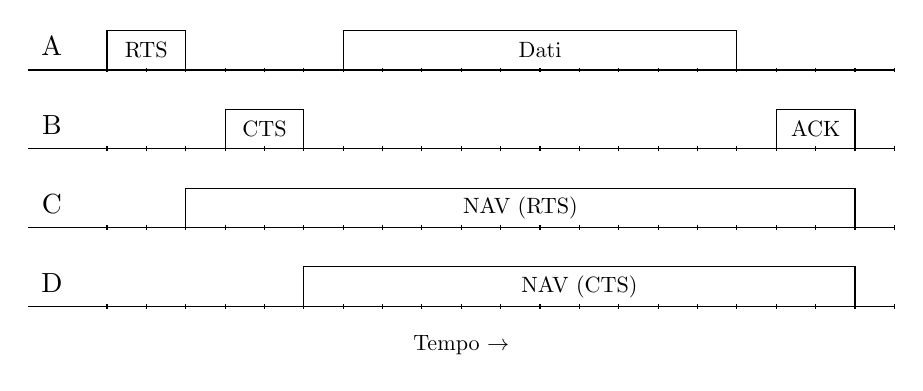
\begin{tikzpicture}
        %%%%%%%%%% Assi %%%%%%%%%%
        \foreach \y in {0,...,3}
            \draw (0,\y) -- ++(11,0);

        \node at (.3,3.3) {A};
        \node at (.3,2.3) {B};
        \node at (.3,1.3) {C};
        \node at (.3,0.3) {D};

        \foreach \y in {-0.03,.97,...,2.97}
            \foreach \x in {1,1.5,...,11}
                \draw (\x,\y) -- ++(0,.06);

        %%%%%%%%% Blocchi %%%%%%%%
        \draw (1,3) -- ++(0,.5) -- ++(1,0) -- ++(0,-0.5);
        \draw (4,3) -- ++(0,.5) -- ++(5,0) -- ++(0,-0.5);
        \draw (2.5,2) -- ++(0,.5) -- ++(1,0) -- ++(0,-0.5);
        \draw (9.5,2) -- ++(0,.5) -- ++(1,0) -- ++(0,-0.5);
        \draw (2,1) -- ++(0,.5) -- ++(8.5,0) -- ++(0,-0.5);
        \draw (3.5,0) -- ++(0,.5) -- ++(7,0) -- ++(0,-0.5);

        %%%%%%%%% Testo %%%%%%%%%%
        \node[scale=0.8] at (1.5,3.25) {RTS};
        \node[scale=0.8] at (6.5,3.25) {Dati};
        \node[scale=0.8] at (3,2.25) {CTS};
        \node[scale=0.8] at (10,2.25) {ACK};
        \node[scale=0.8] at (6.25,1.25) {NAV (RTS)};
        \node[scale=0.8] at (7,.25) {NAV (CTS)};
        \node[scale=0.8] at (5.5,-0.5) {Tempo $\rightarrow$};
    \end{tikzpicture}
\end{center}

            La stazione che deve trasmettere (T) valuta se il mezzo è libero consultando sia NAV che il mezzo reale.

            Se il canale è considerato libero per un determinato intervallo di tempo (\textbf{DIFS}) emette un RTS, altrimenti avvia la procedura di Backoff Esponenziale Binario.

            Quando il ricevente (R) riceve l'RTS risponde con un CTS.

            Se T non riceve il CTS avvia la procedura di Backoff con tempo raddoppiato, altrimenti inizia la trasmissione.

            Se T non riceve un ACK entro un tempo stabilito deve ripetere la procedura, altrimenti il trasferimento è considerato concluso con successo.

    \subsection{Standard IEEE 802}
        \textbf{IEEE (Institute of Eletrical and Eletronic Engineers)}, è un'organizzazione professionale con scopo di ricerche ed applicazioni in vari campi ingegneristici, essa definisce standard in campi elettronici ed informatici.

        Il numero "802" è il primo numero libero negli standard IEEE al momento della formazione del comitato, creato nel 1980 per la standardizzazione delle reti LAN.

        IEEE 802 separa le funzionalità del livello data link in due sottolivelli distinti:
        \begin{itemize}
            \item Sottolivello \textbf{MAC (Medium Access Control)}: gestisce l'accesso al mezzo mediante protocolli di accesso multiplo, quali ad esempio 802.3 (Ethernet), 802.11 (LAN Wireless), 802.15 (Bluetooth), 802.16 (WiMax).
            \item Sottolivello \textbf{LLC (802.2)}: aggiunge un'intestazione contenente codifica del protocollo che ha generato il Frame e a cui è destinato; numero di sequenza e ACK consentendo di operare in tre modalità distinte:
            \begin{itemize}
                \item datagramma inaffidabile
                \item datagramma con ACK
                \item servizio affidabile orientato alle connessioni
            \end{itemize}
        \end{itemize}

    \subsection{Ethernet}
        È la tecnologia dominante per le LAN; ideata a metà degli anni '70 da Bob Metcalfe.
    
        Un \textbf{segmento} Ethernet si realizza con un cavo coassiale di lunghezza fino a 500 m, con un impedenza di 50 $\Omega$.
    
        I terminatori connessi alla fine del segmento assorbono il segnale ed impediscono che rimbalzi ed interferisca con altri segnali.
    
        Nella versione Ethernet 2.0 (1980) la velocità era di 10 Mb/s su cavo coassiale.

        Nel 1983, Ethernet venne recepita da IEEE con il nome di 802.3.

        Il servizio di invio frame è senza riscontro e senza connessione. Per rendere Ethernet più veloce, il servizio è \textbf{Best Effort}, inaffidabile: se il ricevente rileva un errore di trasmissione scarta il pacchetto.

        \subsubsection{Protocollo Ethernet}
            Protocollo di accesso al mezzo: CSMA/CD 1-persistente con algoritmo di Backoff esponenziale binario:
            \begin{itemize}
                \item Se il canale è libero trasmette il frame.
                \begin{itemize}
                    \item Mentre trasmette ascolta il canale, se durante la trasmissione non rivela segnali diversi considera il frame spedito.
                    \item Se durante la trasmissione rivela segnali diversi arresta immediatamente la trasmissione e invia un breve segnale di disturbo (\textbf{jamming sequence}) di 32 bit, quindi entra nella fase di attesa esponenziale prima di riprovare (random tra $2^i - 1$ slots dopo i collisioni). Vengono inviati almeno 96 bit: 64 di preambolo e 32 di disturbo. Il tempo di 96 bit rappresenta il tempo minimo di attesa tra un due frame \textbf{IFG (InterFrame Gap)}.
                    \item Dopo 10 collisioni l'intervallo rimane congelato ($2^{10} - 1 = 1023$ slots).
                    \item Dopo 16 collisioni il controller rinuncia e segnala un errore.
                \end{itemize}
                \item Se il canale è occupato aspetta fino a quando la linea diventa inattiva, poi trasmette.
            \end{itemize}

            Utilizza la \textit{codifica Manchester} opera in \textit{banda base} del livello fisico. Occupa una banda doppia rispetto alla codifica binaria (per avere 10 Mb/s occorre una clock a 20 Mb/s).

            La codifica \textbf{Manchester Differenziale} (usata da 802.5 - Token Ring) è più complessa da realizzare ma offre una maggiore immunità ai rumori.

        \subsubsection{Formato dei frame}
            \begin{center}
    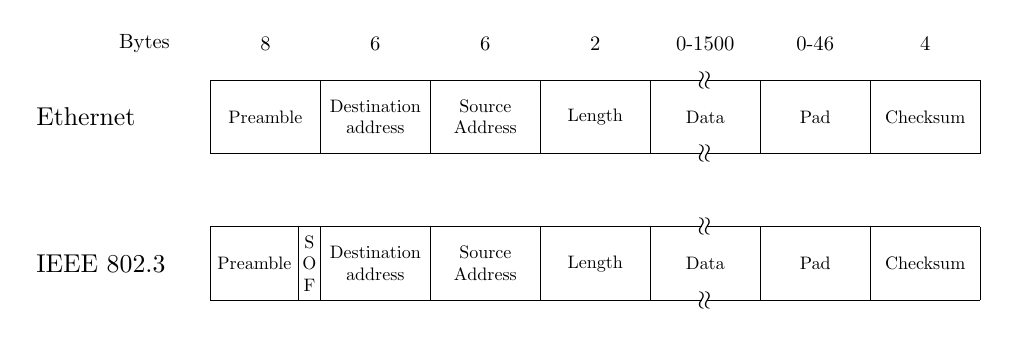
\begin{tikzpicture}[scale=0.931,every node/.style={scale=0.931}]
        %%%%%%% Blocchi 1 %%%%%%%%
        \draw (0,0) -- ++(6.7,0) ++ (.08,0) -- (10.5,0);
        \draw (0,1) -- ++(6.7,0) ++ (.08,0) -- (10.5,1);
        \node[rotate=90] at (6.75,0) {$\approx$};
        \node[rotate=90] at (6.75,1) {$\approx$};
        \draw (1.2,0) -- ++(0,1);

        \foreach \x in {0,1.5,...,10.5}
            \draw (\x,0) -- ++(0,1);

        %%%%%%% Blocchi 2 %%%%%%%%
        \draw (0,2) -- ++(6.7,0) ++ (.08,0) -- (10.5,2);
        \draw (0,3) -- ++(6.7,0) ++ (.08,0) -- (10.5,3);
        \node[rotate=90] at (6.75,2) {$\approx$};
        \node[rotate=90] at (6.75,3) {$\approx$};

        \foreach \x in {0,1.5,...,10.5}
            \draw (\x,2) -- ++(0,1);

        %%%%%%% Tipo frame %%%%%%%
        \node[anchor=west] at (-2.5,2.5) {Ethernet};
        \node[anchor=west] at (-2.5,0.5) {IEEE 802.3};

        %%%%%%%% Testo 1 %%%%%%%%%
        \node[scale=0.7] at (.6,.5) {Preamble};
        \node[scale=0.7,text width=0.27cm,align=center] at (1.35,.5) {S O F};
        \node[scale=0.7,text width=2cm,align=center] at (2.25,.5) {Destination address};
        \node[scale=0.7,text width=2cm,align=center] at (3.75,.5) {Source Address};
        \node[scale=0.7,text width=2cm,align=center] at (5.25,.5) {Length};
        \node[scale=0.7,text width=2cm,align=center] at (6.75,.5) {Data};
        \node[scale=0.7,text width=2cm,align=center] at (8.25,.5) {Pad};
        \node[scale=0.7,text width=2cm,align=center] at (9.75,.5) {Checksum};

        %%%%%%%% Testo 2 %%%%%%%%%
        \node[scale=0.7] at (.75,2.5) {Preamble};
        \node[scale=0.7,text width=2cm,align=center] at (2.25,2.5) {Destination address};
        \node[scale=0.7,text width=2cm,align=center] at (3.75,2.5) {Source Address};
        \node[scale=0.7,text width=2cm,align=center] at (5.25,2.5) {Length};
        \node[scale=0.7,text width=2cm,align=center] at (6.75,2.5) {Data};
        \node[scale=0.7,text width=2cm,align=center] at (8.25,2.5) {Pad};
        \node[scale=0.7,text width=2cm,align=center] at (9.75,2.5) {Checksum};

        %%%%%%%%% Bytes %%%%%%%%%%
        \node[scale=0.8] at (-0.9,3.5) {Bytes};
        \node[scale=0.8] at (0.75,3.5) {8};
        \node[scale=0.8] at (2.25,3.5) {6};
        \node[scale=0.8] at (3.75,3.5) {6};
        \node[scale=0.8] at (5.25,3.5) {2};
        \node[scale=0.8] at (6.75,3.5) {0-1500};
        \node[scale=0.8] at (8.25,3.5) {0-46};
        \node[scale=0.8] at (9.75,3.5) {4};
    \end{tikzpicture}
\end{center}

            Il campo \textbf{preambolo} contiene 7 (o 8) sequenze di 10101010 ovvero un'onda quadra di circa 5 ms che consente al ricevitore di sincronizzarsi.

            Il campo \textbf{SoF (Start of Frame)} indica l'inizio di un frame: contiene la sequenza 10101011, gli ultimi 2 bit a 1, indicano che il prossimo bit sarà il primo del frame.

            Il campo \textbf{Type/Length} contiene il codice del protocollo di livello superiore che ha generato il frame. Nello standard IEEE 802.3, il campo \textit{Type} è sostituio dal campo \textit{Length}, che contiene il numero di byte del campo \textit{Data}. I due standard possono coesistere.

            Gli indirizzi Ethernet sono di 6 byte, (248 possibili indirizzi), l'indirizzo viene scritto nel firmware del controller di rete ed è unico.

            I primi 3 byte identificano il \textit{Vendor}: negli indirizzi unicast il primo byte è pari, negli indirizzi multicast il primo byte è dispari. L'indirizzo di broadcast è \texttt{ff-ff-ff-ff-ff-ff}.

            Il campo \textbf{Data} contiene le PDU dei livelli superiori.

            Il campo \textbf{FCS} contiene il valore di CRC-32.

            Il marcatore di fine frame manca, e tale ruolo è assunto dal \textit{IFG (Inter Frame Gap)} il cui valore minimo è di 96 bit.

            Un adattatore Ethernet accetta i pacchetti nei seguenti casi:
            \begin{itemize}
                \item Tutti i frame broadcast.
                \item I frame unicast indirizzati all'interfaccia.
                \item I frame di un particolare indirizzzo multicast, se l'interfaccia è stata configurata oppurtunamente.
                \item Tutti i frame se l'interfaccia è configurata in modo promiscuo.
            \end{itemize}

        \subsubsection{Dimensione del frame e slot time}
            La \textbf{massima dimensione} di dati trasportabili da un servizio Data-Link è detta \textbf{MTU (Maximum Transfer Unit)}.

            L'MTU di Ethernet è di 1500 byte.

            La minima dimensione è di 64 byte (46 payload e 18 header) = 512 bit. Per 512 bit, abbiamo $L$ = 10 [Km].

            La durata minima di un frame è quindi di $t$ = 51.2 [$\mu s$], che rappresentano lo \textbf{Slot Time} (questo è anche il tempo utile per rilevare una collisione, per cui in questo tempo il frame deve aver percorso in andata e ritorno l'intera rete).

        \subsubsection{Evoluzione dello standard: Ethernet}
            \subsubsection*{1980: Ethernet}
            Intel e Xerox rilasciano le specifiche di Ethernet 2.0 che rappresenta lo standard per le LAN. Utilizza una topologia a bus su cavo coassiale a 10 Mb/s.
        
            Non ha bisogno di apparati di rete, ma è impossibile la gestione centralizzata.
        
            \subsubsection*{1983: IEEE 802.3}
            Ethernet diventa uno standard ufficiale con il nome di IEEE 802.3, utilizza la codifica Manchester con un clock a 20 MHz su doppino.

            Per avere una connessione full-duplex, si utilizzano due doppini: questo permette di raddoppiare la capacità trasmissiva 20 Mb/s.

            Il doppino è un canale punto-punto, quindi è necessaria una topologia a stella con un apparato concentratatore (\textit{hub}).

            \subsubsection*{1995: IEEE 802.3u}
            Chiamato anche \textbf{Fast Ethernet}, tramite l'utilizzo di doppini di categoria 5, ed un clock di 125 Mhz, permette di raggiungere una velocità di 100 Mb/s.

            \subsubsection*{1999: IEEE 802.3z}
            Lo standard che utilizza è il \textbf{1000baseT}, che utilizza un doppino di categoria (almeno) 5, (massimo 100 metri).

            Si usano tutte le quattro coppie, ogni coppia trasporta 250 Mb/s, il baud-rate è ancora 125 M (come Fast Ethernet), ma utilizza la codifica PAM5 (modulazione di ampiezza di una portante, usa 5 simboli con 2 bit per baud).

            Nella modalità half-duplex, abbiamo 500 Mb/s per direzione, mentre nella modalità full-duplex si può arrivare a 1 G/s.

            Quindi abbiamo che:
            \begin{itemize}
                \item \textbf{Modalità full duplex [1 Gb/s]}: tutte le configurazioni Gigabit Ethernet sono punto-punto abbandonando il sistema multi-accesso di Ethernet originale, utilizza solo Ethernet Switch, che bufferizzando i frame del pacchetto in modo da eliminare le collisioni ed il conseguente limite sulla durata del pacchetto. La lunghezza massima del cavo è stabilita dall'attenuazione del segnale.
                \item \textbf{Modalità half duplex [500 Mb/s]}: usato solo per mantenere la compatibilità con il protocollo CSMA/CD delle precedenti versioni.
                Per risolvere il problema del rilevamento delle collisioni vengono introdotte due estensioni:
                \begin{itemize}
                    \item \textbf{Carrier extension}: consente di aumentare il Padding, portando il frame minimo a 512 byte (slot time da 4.1 $\mu s$).
                    \item \textbf{Frame bursting}: consente di aggregare più frame in uscita, in modo da raggiungere 512 byte (max. 64 Kb).
                \end{itemize}
            \end{itemize}

            \subsubsection*{2005: 10GbE}
            10 Gb Ethernet (10GbE) è stato inizialmente introdotto solo per fibra ottica, nel 2009 è stato esteso al doppino.

            Permette appunto di raggiungere la velocità di 10 Gb/s.

            Lo standard è solo switched full-duplex, quindi non è utilizzato CDMA/CD. Nella codifica i bit vengono mischiati, poi si applica 64B/66B (per evitare lunghe sequenze di 0 o 1.

    \subsection{Dispositivi LAN}
        \subsubsection{Ethernet Repeater}
            Il \textit{repeater} è un nodo di transito che agisce a livello fisico, connettendo due o più segmenti Ethernet.
        
            I bit ricevuti da un'interfaccia vengono rigenerati e replicati sulle altre. Ethernet stabilisce in una rete, un massimo di 4 repeater ed una distanza mas- sima di 2.5 Km.

            \begin{center}
                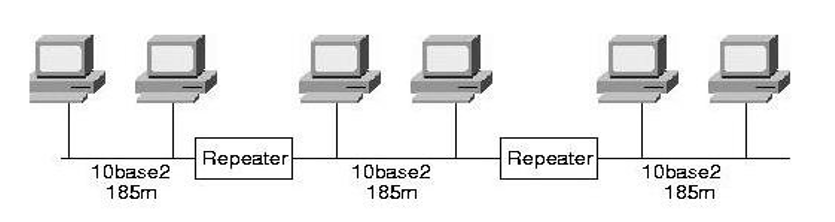
\includegraphics[scale=0.4]{chapters/3/assets/schema_p.png}
            \end{center}

        \subsubsection{Ethernet Hub}
            Un \textit{hub} è un repeater con più di due interfacce Ethernet.
            
            L'Hub permette di realizzare un rete broadcast utilizzando canali punto-punto. L'hub estende sia il dominio di collisioni, che il dominio di broadcast.

            \begin{center}
                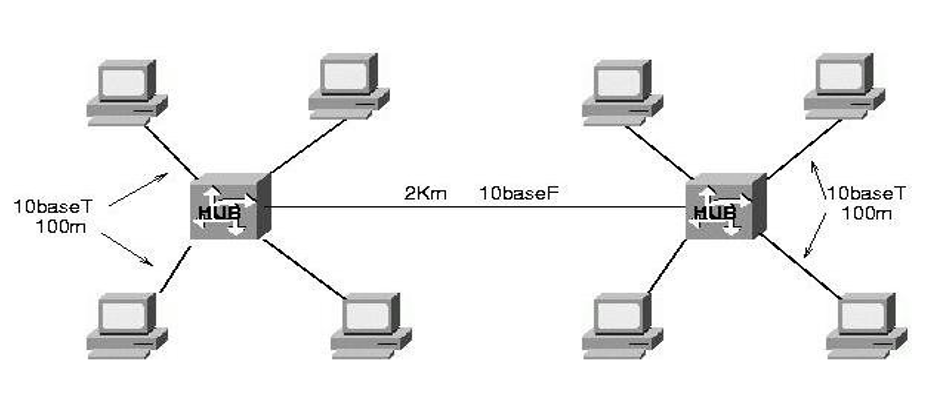
\includegraphics[scale=0.36]{chapters/3/assets/schema_q.png}
            \end{center}

        \subsubsection{Commutazione livello data link: Bridge}
            A differenza dell'hub il \textbf{bridge} effettua l'operazione di \textbf{filtering}: ritrasmette solamente i pacchetti che devono transitare da una LAN ad un'altra ed i pacchetti broadcast. In questo modo vengono separati i domini di collisione (ma non quelli di broadcast).
        
            L'instradamento (\textbf{forwarding}) avviene in base ad una tabella dei bridge in cui sono indicati gli indirizzi MAC dietro ad ogni interfaccia.

            \begin{center}
    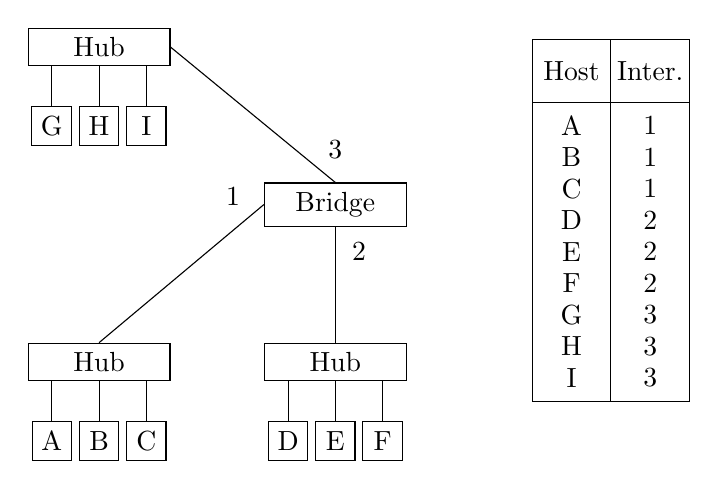
\begin{tikzpicture}
        %%%%%%%%%% Hubs %%%%%%%%%%
        \node[draw,rectangle,minimum width=1.8cm] (Hub1) at (0,0) {Hub};
        \node[draw,rectangle,minimum width=1.8cm] (Hub2) at (3,0) {Hub};
        \node[draw,rectangle,minimum width=1.8cm] (Hub3) at (0,4) {Hub};

        %%%%%%%%% Bridge %%%%%%%%%
        \node[draw,rectangle,minimum width=1.8cm] (Bridge) at (3,2) {Bridge};

        %%%%%%%% Clients %%%%%%%%%
        \node[draw,rectangle,minimum width=0.5cm,minimum height=0.5cm] (A) at (-0.6,-1) {A};
        \node[draw,rectangle,minimum width=0.5cm,minimum height=0.5cm] (B) at (0,-1) {B};
        \node[draw,rectangle,minimum width=0.5cm,minimum height=0.5cm] (C) at (0.6,-1) {C};
        \node[draw,rectangle,minimum width=0.5cm,minimum height=0.5cm] (D) at (2.4,-1) {D};
        \node[draw,rectangle,minimum width=0.5cm,minimum height=0.5cm] (E) at (3,-1) {E};
        \node[draw,rectangle,minimum width=0.5cm,minimum height=0.5cm] (F) at (3.6,-1) {F};
        \node[draw,rectangle,minimum width=0.5cm,minimum height=0.5cm] (G) at (-0.6,3) {G};
        \node[draw,rectangle,minimum width=0.5cm,minimum height=0.5cm] (H) at (0,3) {H};
        \node[draw,rectangle,minimum width=0.5cm,minimum height=0.5cm] (I) at (0.6,3) {I};

        %%%%%%%%% Links %%%%%%%%%%
        \draw (Hub1.north) -- (Bridge.west);
        \draw (Hub2.north) -- (Bridge.south);
        \draw (Hub3.east) -- (Bridge.north);
        \draw (A.north) -- ++(0,0.5);
        \draw (B.north) -- ++(0,0.5);
        \draw (C.north) -- ++(0,0.5);
        \draw (D.north) -- ++(0,0.5);
        \draw (E.north) -- ++(0,0.5);
        \draw (F.north) -- ++(0,0.5);
        \draw (G.north) -- ++(0,0.5);
        \draw (H.north) -- ++(0,0.5);
        \draw (I.north) -- ++(0,0.5);

        %%%%%%%%% Porte %%%%%%%%%%
        \node at (1.7,2.1) {1};
        \node at (3.3,1.4) {2};
        \node at (3,2.7) {3};

        %%%%%%%% Tabella %%%%%%%%%
        \draw (5.5,-0.5) -- ++(2,0);
        \draw (5.5,3.3) -- ++(2,0);
        \draw (5.5,4.1) -- ++(2,0);
        \draw (5.5,-0.5) -- ++(0,4.6);
        \draw (6.5,-0.5) -- ++(0,4.6);
        \draw (7.5,-0.5) -- ++(0,4.6);
        \node at (6,3) {A};
        \node at (6,2.6) {B};
        \node at (6,2.2) {C};
        \node at (6,1.8) {D};
        \node at (6,1.4) {E};
        \node at (6,1) {F};
        \node at (6,0.6) {G};
        \node at (6,0.2) {H};
        \node at (6,-0.2) {I};
        \node at (7,3) {1};
        \node at (7,2.6) {1};
        \node at (7,2.2) {1};
        \node at (7,1.8) {2};
        \node at (7,1.4) {2};
        \node at (7,1) {2};
        \node at (7,0.6) {3};
        \node at (7,0.2) {3};
        \node at (7,-0.2) {3};

        \node at (6,3.7) {Host};
        \node at (7,3.7) {Inter.};
    \end{tikzpicture}
\end{center}

            La tabella del bridge è costruita automaticamente in modo autonomo:
            \begin{itemize}
                \item All'accensione del bridge la tabella è vuota.
                \item Quando arriva un frame, l'indirizzo del mittente viene scritto nella tabella, associato all'interfaccia di provenienza ed al tempo attuale. Se l'indirizzo di destinazione non è presente in tabella, il frame viene inoltrato su tutte le interfacce tranne quella di provenienza (\textbf{flooding}), altrimenti, viene inoltrato sulla sola interfaccia indicata in tabella.
                \item Il bridge cancella un indirizzo della tabella, se per un certo periodo di tempo (aging time) non riceve alcun frame con quell'indirizzo di provenienza.
            \end{itemize}

            I bridge sono comunemente utilizzati per collegare due o più LAN distinte.

            Se le LAN sono remote (in diverse edifici o diverse città) i bridge vengono collegati mediante linee punto-punto su cui possiamo utilizzare protocolli punto-punto (PPP) ed incapsulare al suo interno il frame MAC, oppure possiamo usare la linea punto-punto direttamente con protocollo MAC.

            In ogni caso il bridge non cambia gli indirizzi fisici del frame.

            Ogni LAN ha un proprio formato dei frame, quindi se il MTU della LAN di destinazione è troppo piccolo, i bridge devono eliminare il frame (la frammentazione è prevista solo a livello rete).

            Se la LAN di provenienza è cifrata (WiFi), il bridge deve essere in grado di decifrare prima di inoltrare.

        \subsubsection{Ethernet commutata: Switch}
            Lo \textbf{switch} è un commutatore di rete a livello 2: i frame che riceve vengono smistati solo sull'interfaccia dove è attestato il destinatario.
            
            Sono sostanzialmente dei bridge ad alte prestazioni con interfacce multiple. I vantaggi di uno Switch sono:
            \begin{itemize}
                \item Aumento del throughput sotto carico: uno switch a $N$ porte può essere attraversato contemporaneamente da $\frac{N}{2}$ connessioni.
                \item Ogni connessione può essere full-duplex, quindi raddoppia il throughput.
                \item Sicurezza: sull'interfaccia di un terminale non transitano frame di altre connessioni.
                \item I segmenti diventano domini di collisione separati o privi di connessione (Switch-PC).
            \end{itemize}

            Gli switch hanno una tabella interna con le associazioni MAC-Interfaccia. Lo switch costruisce la tabella leggendo gli indirizzi dai frame che lo attraversano: se il mittente di un frame non è in tabella viene inserito, se il destinatario non è in tabella o è broadcast (\texttt{ff-ff-ff-ff-ff-ff}) il frame viene inviato a tutti (flooding).

            La commutazione è realizzata da dispositivi hardware denominati \textit{Crossbar Switch}.

            Esistono due tipi di Switch:
            \begin{itemize}
                \item Switch \textbf{store-and-forward}: il frame viene ricevuto interamente poi ritrasmesso: consente l'utilizzo di velocità eterogenee. Assenza di collisioni.
                \item Switch \textbf{cut-through}: l'indirizzo di destinazione viene analizzato mentre il frame sta entrando nello switch. Se il link di uscita è libero il frame viene instradato sull'interfaccia di uscita senza bufferizzazione, dopo che sono stati letti i primi 14 byte (circa 25 $\mu s$ per Ethernet e 7 $\mu s$ per Fast Ethernet).
            \end{itemize}

            Tempi di latenza bassi, ma vengono inoltrati anche frame corrotti e si estende il dominio di collisione.
    
            Funzionalità non presente nei bridge.

        \subsubsection{Spanning Tree}
            In una LAN composta da bridge e/o switch, possiamo avere una topologia magliata per due possibili motivi:
            \begin{itemize}
                \item Progetto di ridondanza: garantire percorsi alternativi in caso di guasti.
                \item Errori di configurazione.
            \end{itemize}

            La presenza di una topologia ad anello, potrebbe portare a situazioni in cui i frame circolano all'infinito.

            Si tratta quindi di rendere aciclico un grafo connesso con archi pesati non orientati, isolando in modo opportuno alcuni archi.

            Il metodo utilizzato nelle LAN consiste nel determinare un albero ricoprente (\textbf{spanning tree}) sopra il grafo.

            L'algoritmo che determina l'albero e isola gli archi eccedenti nelle LAN è detto \textbf{STP (Spanning Tree Protocol)}.

        \subsubsection{Spanning Tree Protocol}
            Le funzionalità dell'algoritmo sono:
            \begin{itemize}
                \item Deve intervenire nel più breve tempo possibile.
                \item Deve introdurre un overhead minimo.
                \item Deve essere flessibile, cioè deve poter ammettere che un bridge venga aggiunto successivamente ad una rete configurata, senza che sia necessario riconfigurare tutta la rete.
            \end{itemize}

            L'algoritmo distribuito STP è stato standardizzato nel 2010 con il nome di \textbf{IEEE 802.1D}.

            Il protocollo si basa sullo scambio di frame (detti \textbf{BPDU: Bridge Protocol Data Unit}) tra i Bridge del dominio di broadcast utilizzando l'indirizzo multicast \texttt{01:80:C2:00:00:00}.

            Ci sono tre tipi di BPDU:
            \begin{itemize}
                \item  \textbf{Configuration BPDU}, usati per il calcolo della configurazione del protocollo.
                \item \textbf{Topology Change Notification} e \textbf{Topology Change Notification Ack} usati per annunciare un cambiamento della topologia.
            \end{itemize}

            L'algoritmo opera nei seguenti passi:
            \begin{enumerate}
                \item Elezione del \textbf{Root-Bridge}: ogni bridge ha un proprio identificativo (ID) che spedisce in multicast in modo che tutti i Bridge sappino chi è il bridge con l'ID più piccolo. Questo bridge diventa la radice dell'albero.
                \item Selezione della \textbf{Root-Door}: per ogni bridge si seleziona la porta più conveniente per interconnetterlo al root.
                \item Selezione del \textbf{Designated-Bridge}: per ogni LAN si sceglie quale bridge è designato ad interconnetterla con il root, la porta utilizzata è la \textbf{Designated-Door}. Al termine di queste azioni, lo spanning procede alla messa in stato di blocking, per tutte le porte che non sono Root-Door o Designated-Door.
            \end{enumerate}

            \begin{center}
                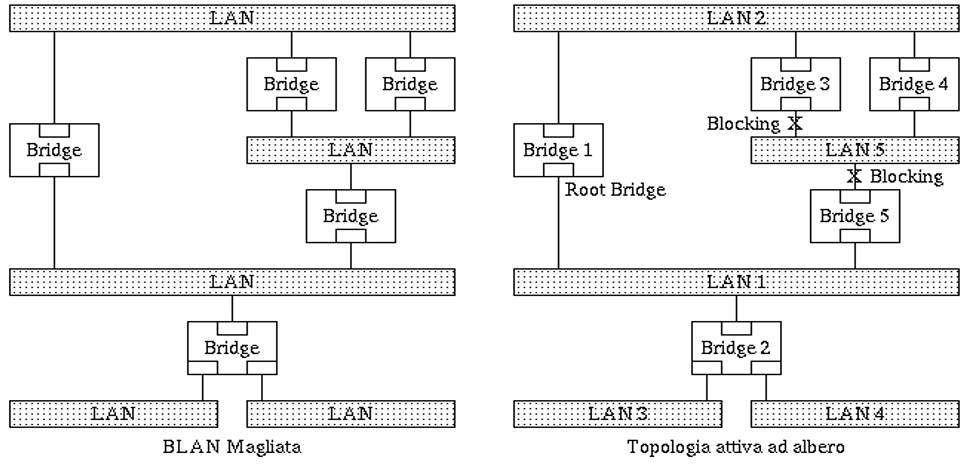
\includegraphics[scale=0.35]{chapters/3/assets/schema_s.png}
            \end{center}

        \subsection{Virtual LAN (VLAN)}
            Le \textbf{VLAN (Virtual LAN)} sfruttano la capacità di inoltro intelligente degli switch.
        
            Permettono di costruire su un'unica infrastruttura fisica più LAN logicamente separate.
        
            I vantaggi di una VLAN sono:
            \begin{itemize}
                \item Limitano il traffico di broadcast all'interno della singola VLAN.
                \item Permettono la progettazione logica della rete indipendentemente dalla dislocazione fisica delle stazioni.
                \item Aumentano il livello di sicurezza della rete confinando il traffico interno di ogni VLAN alle sole stazioni appartenenti ad essa.
            \end{itemize}
        
            I \textbf{VLAN-Switch} sono switch che supportano la gestione VLAN mediante opportune tabelle di configurazione in cui sono elencate le VLAN disponibili e le porte associate.

            Ad una porta possono essere associate più VLAN (se dietro la porta c'è un hub o uno switch).

            Le trame che attraversano diversi switch devono essere etichettate per consentirne una corretta gestione. Occorre quindi una modifica dell'header del frame per far posto all'etichetta VLAN.

            Il primo switch che tocca il frame aggiunge l'etichetta e l'ultimo sul percorso la rimuove. 802.1Q è lo standard proposto nel 1998 da IEEE per la modifica del Frame Ethernet.

            \begin{center}
                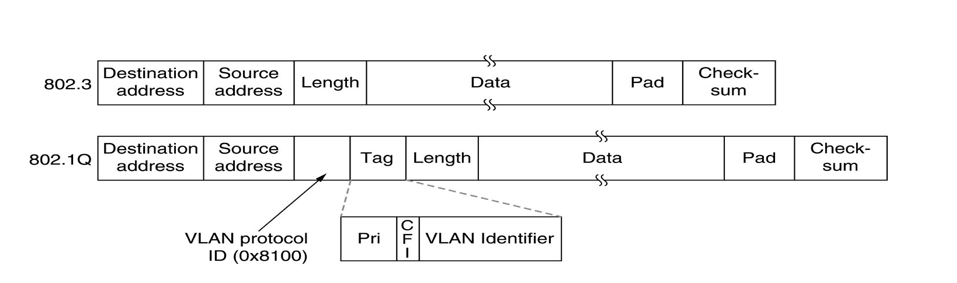
\includegraphics[scale=0.35]{chapters/3/assets/schema_t.png}
            \end{center}

        \subsubsection{Criteri di appartenza alle VLAN}
            L'appartenenza ad un host ad una VLAN può essere definita secondo vari criteri:
            \begin{itemize}
                \item Porte: ciascuna porta di uno switch è configurata per appartenere ad una data VLAN.
                \item Autenticazione: diversi apparati possono essere assegnati automaticamente ad una VLAN sulla base di criteri di autenticazione (es. Access Point WiFi).
                \item Protocollo: ad esempio i pacchetti IP possono appartenere ad una VLAN, diversa da quella usata dai pacchetti IPX.
            \end{itemize}

    \subsection{Wireless}
        Le famiglie di protocolli \textit{wireless} sono:
            \begin{itemize}
                \item 802.11: Wireless LAN (WiFi)
                \item 802.16: Wireless MAN (WiMax)
                \item 802.15: Wireless PAN (Bluetooth)
            \end{itemize}

        Le reti Wireless hanno due possibili modalità di utilizzo:
        \begin{itemize}
            \item con infrastruttura: ogni client è associato ad una stazione base (bridge).
            \item reti ad hoc: reti di computer associati tra loro.
        \end{itemize}

        \subsubsection{802.11: Wireless LAN}
            Le LAN Wireless hanno minori prestazioni e maggiori costi rispetto alle LAN Wired, per cui non sono alternative, ma coprono nuove, diverse esigenze.
        
            Il canale è multi-accesso per cui il throughput è condiviso.
    
            Il sotto-strato MAC è definito dallo standard 802.11 con 6 diverse tecniche di trasmissione (Infrared, HDSS, DSSS, OFDM, HR-DSSS e OFDM). Dal 1997 ad oggi sono stati realizzati diversi protocolli che utilizzano queste tecniche: 802.11, 802.11a 802.11b, 802.11g, 802.11n, 802.11ac
        
            Tutte le implementazioni (eccetto gli infrarossi in 802.11) operano nelle frequenze ISM.

        \subsubsection{Lo stato fisico di 802.11}
            Publlicato nel 1997, 802.11 è il protocollo originale.
        
            Aveva una velocità limitata di 1 o 2 Mb/s con tre varianti tecniche:
            \begin{itemize}
                \item Infrarosso: non penetra i muri ed è sensibile alla luce solare.
                \item Frequency Hopping Spread Spectrum (FHSS).
                \item Direct Sequence Spread Spectrum (DSSS).
            \end{itemize}
            
        \subsubsection{Lo stato fisico di 802.11a}
            Pubblicato nel 1999 utilizza 8 canali da 20 MHz, attorno a 5.2 GHz raggiungendo una velocità di 54 Mb/s (25/31 reali).
        
            La tecnica utilizzata per la codifica è la OFDM: ogni canale da 20 MHz è suddiviso in 52 portanti da 300 KHz, con modulazione di fase (QPSK) e di ampiezza e fase (QAM), come ADSL.

            La trasmissione ortogonale consente di ridurre l'interferenza tra canali adiacenti parzialmente sovrapposti.
        
        \subsubsection{Lo stato fisico di 802.11b}
            Pubblicato nel 1999, 802.11b opera a 2.4 GHz con la tecnica di modulazione HR-DSSS, ha una velocità dichiarata di 11 Mb/s ma il protocollo MAC CSMA/CA introduce un overhead che ne dimezza la velocità reale (5.9 Mb/s).

            Se il segnale è debole, la velocità massima può essere ridotta a 2 Mb/s o 1 Mb/s, funzionano in DSSS per combatibilità con 802.11.

            Lo spettro è suddiviso in 14 canali da 22 MHz parzialmente sovrapposti.

            Per evitare interferenze vengono generalmente utilizzati due gruppi di canali quando ci sono diverse reti WiFi.

        \subsubsection{Lo stato fisico di 802.11g}
            Pubblicato nel 2003 utilizza la frequenza di 802.11b, con cui è backward-compa\-tible, e la modulazione OFDM su 52 portanti come 802.11a, ma utilizza i 14 canali da 22 MHz attorno a 2.4 GHz di 802.11b.

            La velocità è di 54 Mb/s (24 Mbps reali).
        
        \subsubsection{Lo stato fisico di 802.11n}
            La versione definitiva dello standard è stata ratificata nel 2009.
        
            Opera a 2.4 e 5.4 GHz con canali raddoppiati (20 o 40 MHz), utilizza OFDM con modulazione 64-QAM.
        
            Altri miglioramenti rispetto a 802.11g grazie alla tecnologia \textbf{MIMO (Multiple Input Multiple Output)}, si utilizzano fino a 4 antenne per trasmettere fino a 4 flussi radio paralleli oppure per migliorare il raggio di copertura.

        \subsubsection{Lo stato fisico di 802.11ac}
            La versione definitiva dello standard è stata ratificata nel 2014.
        
            Rispetto a 802.11n opera solo a 5 GHz con canali più larghi (80 o 160 MHz), più antenne MIMO (fino a 8) e una modulazione fino a 256-QAM.

            La velocità massima per flusso (banda 160Mhz, 256-QAM, un'antenna MIMO) è di circa 800 Mb/s (throughput 600 Mb/s).

    \subsection{Il protocollo MAC di 802.11}
        Il protocollo copre tre funzioni:
        \begin{itemize}
            \item Consegna affidabile dei frame.
            \item Controllo dell'accesso.
            \item Sicurezza.
        \end{itemize}
        
        Fornisce due modalità di funzionamento:
        \begin{itemize}
            \item A contesa: \textbf{DCF (Distributed Coordination Function)}
            \item Senza contesa: \textbf{PCF (Point Coordination Function}
        \end{itemize}

        \begin{center}
            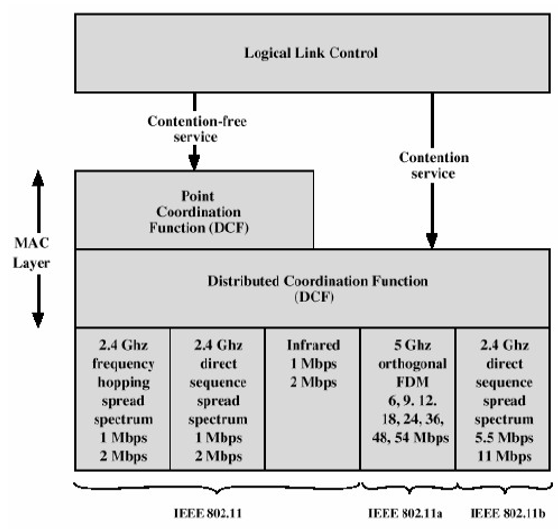
\includegraphics[scale=0.55]{chapters/3/assets/schema_u.png}
        \end{center}

        \subsubsection{Protocolli MAC: Intervali tra frame}
            I protocolli DCF e PCF possono convivere nella stessa cella, grazie ad una opportuna assegnazione dei tempi di attesa (priorità nella risposta):
            \begin{itemize}
                \item \textbf{SIFS (Short Inter Frame Space)}: per separare i frame di una singola trasmissione.
                \item \textbf{PIFS (PCF IFS)}: un eventuale AP può inviare i suoi frame di controllo.
                \item \textbf{DIFS (DCF IFS)}: se l'AP non invia frame, le stazioni possono tentare di acquisire il canale.
            \end{itemize}

            \begin{center}
                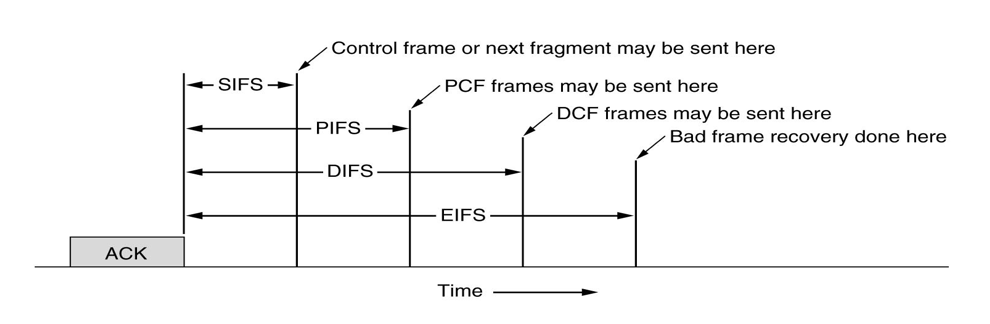
\includegraphics[scale=0.346]{chapters/3/assets/schema_v.png}
            \end{center}

            Il protocollo DCF è a gestione distribuita con CSMA/CA.

            Quando la stazione deve trasmettere manda un RTS, quindi attende il CTS dal destinatario ed invia i frame.

            Per ogni frame inviato attiva un timer e attende un ACK. Se non arriva l'ACK (CRC errato, etc.) il protocollo si ripete.

            Al contrario delle reti wired, le reti wireless sono soggette a rumore e quindi inaffidabili. Se i frame sono troppo lunghi hanno poche probabilità di arrivare intatti a destinazione.

            Per questo 802.11 ammette frammentazione in parti piccole. Una volta acquisito il canale (con RTS e CTS) più frammenti possono essere inviati in sequenza (\textit{fragment burst}), il NAV copre solo il primo frammento, mentre i frammenti successivi sono garantiti dal tempo di SIFS.

            \begin{center}
                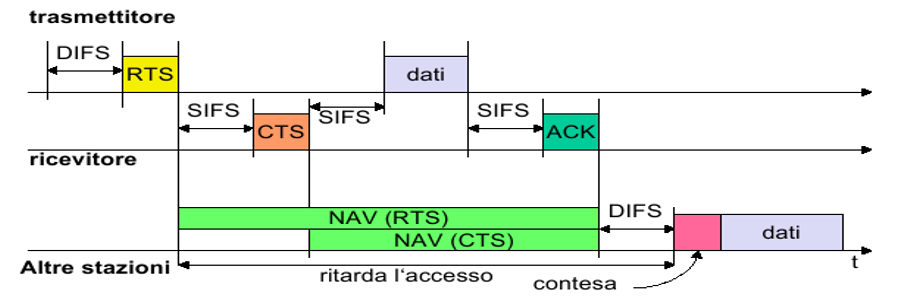
\includegraphics[scale=0.35]{chapters/3/assets/schema_w.png}
            \end{center}

        \subsubsection{Protocollo MAC senza contesa: PCF}
            L'AP gestisce tutte le stazioni della sua cella. Un broadcast (\textit{beacon frame}) viene inviato da 10 a 100 volte al secondo per sincronizzare le stazioni e rappresenta l'invito ad associarsi da parte di nuove stazioni, che rispondono con le caratteristiche della stazione.

            Le stazioni associate vengono abilitate a comunicare in un periodo senza contesa con un meccanismo di polling. Al termine l'AP invia un frame di fine del periodo di nessuna contesa e possono riprendere le contese.

            Tutte le implementazioni supportano DCF, mentre PCF è opzionale.

            \begin{center}
                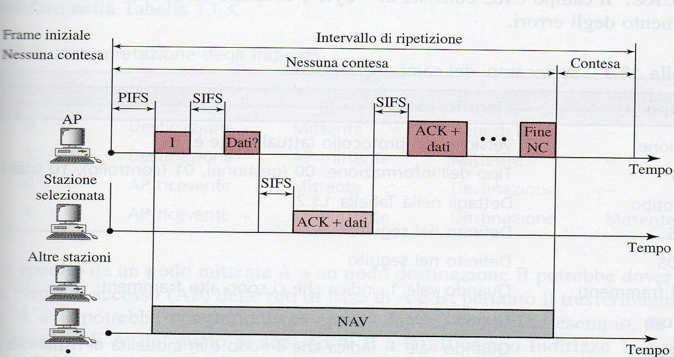
\includegraphics[scale=0.5]{chapters/3/assets/schema_x.png}
            \end{center}

        \subsubsection{Il frame di 802.11}
            Esistono tre tipi di frame:
            \begin{itemize}
                \item Dati
                \item Controllo (RTS, CTS, ACK)
                \item Management
            \end{itemize}

            Campi di un frame:
            \begin{itemize}
                \item \textit{Frame Control}: il primo ottetto è suddiviso in tre campi con il seguente significato:
                \begin{itemize}
                    \item Versione: versione dello standard IEEE 802.11
                    \item Tipo (2 bit): specifica il tipo di frame [Management(00), Controllo(01), Dati(10)].
                    \item Sottotipo (4 bit): RTS (01-1011), CTS (01-1100), ACK (01-1101), Beacon (00-1000)
                \end{itemize}
                Gli altri 8 flag che seguono, se imposti ad 1, hanno il seguente significato:
                \begin{itemize}
                    \item \textbf{To DS}: il frame è diretto al sistema di distribuzione.
                    \item \textbf{From DS}: il frame proviene dal sistema di distribuzione.
                    \item \textbf{More Fragment}: seguono altri frammenti appartenenti allo stesso frame.
                    \item \textbf{Retry}: questo frame è la ripetizione di quello precedente.
                    \item \textbf{Low energy}: la stazione base mette una stazione in stato di sleep.
                    \item \textbf{More Frame}: il trasmettitore ha altri frame per il ricevitore.
                    \item \textbf{WEP}: il campo Dati è stato crittografato con l'algoritmo WEP.
                    \item \textbf{Sorted}: il frammento appartiene alla classe di servizio Strictly-Ordered.
                \end{itemize}
                \item Duration: consentono di provedere per quanto tempo il mezzo resterà occupato.
                \item Address: formato IEEE 802 (48 bit). Il frame dati contiene 4 indirizzi, perché oltre al MAC delle stazioni di origine e di destinazione, sono presenti anche quelli degli AP di entrata e di uscita.
                \item Sequence: consente di numerare i frames.
                \item Data: è il payload lungo fino a 2312 byte: header di 24 byte, massimo totale di 2346 byte, non c'è minimo poiché non è possibile avere collisioni sui dati.
                \item Checksum: CRC-32.
            \end{itemize}

            \begin{center}
                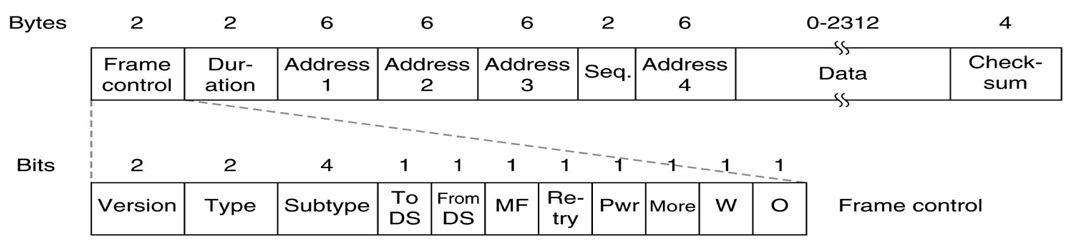
\includegraphics[scale=0.31]{chapters/3/assets/schema_y.png}
            \end{center}

        \subsubsection{MTU e frammentazione}
            Il payload può arrivare fino a 2312 byte, che è quindi il MTU di IEEE 802.11, ma è possibile definire una soglia di frammentazione tra 400 e 2312 byte.
        
            La frammentazione migliora le prestazioni poiché riduce la probabilità di errore, quindi rinvio.

        \subsubsection{Servizi}
            Ogni LAN wireless deve fornire servizi classificabili in due categorie:
            \begin{itemize}
                \item Servizi di distribuzione: forniti dall'AP.
                \item Servizi di stazione: assolti da tutte le stazioni.
            \end{itemize}

            I servizi sono gestiti mediante lo scambio di appositi frame di Management.

            Un frame di Management importante è il \textbf{beacon frame} che viene inviato dall'Access Point ad intervalli regolari (tipicamente 10 al secondo) e contiene l'identificatore della cella.

            In questo modo le stazioni vengono a conoscenza degli Access Point attivi e possono inviare frame di Management per la richiesta di servizi.

            I \textbf{servizi di distribuzione} sono:
            \begin{itemize}
                \item \textbf{Associazione}: appena una stazione entra nel raggio d'azione dell'AP, invoca questo servzio per informare la stazione base della sua presenza e delle sue necessità.
                \item \textbf{Separazione}: sia le stazioni, sia l'AP, possono terminare una precedente associazione; una stazione mobile deve invocare questo servizio prima di spegnersi o lasciare la cella.
                \item \textbf{Riassocazione}: una stazione in moto può trasferire il controllo da un AP ad un altro.
                \item \textbf{Distribuzione}: l'AP smista i frame che lo raggiungono verso le stazioni della propria cella o verso gli AP, attraverso un sistema di distribuzione (rete cablata).
                \item \textbf{Integrazione}: gestisce la traduzione dei frame 802.11 verso altri formati.
            \end{itemize}

            I \textbf{servizi di stazione} sono:
            \begin{itemize}
                \item \textbf{Autenticazione}: una stazione deve autenticarsi per evitare che i frame arrivino a stazioni non autorizzate. Dopo l'associazione, la base invia un \textit{Frame Challenge} a cui la stazione deve rispondere con frame per l'autenticazione.
                Ci sono due tipi di autenticazione:
                \begin{itemize}
                    \item \textbf{A sistema aperto}: nessuna sicurezza.
                    \item \textit{A chiave condivisa}: l'AP condivide con tutte le stazioni una chiave segreta. L'AP invia una stringa di prova (Challenge), la stazione codifica il Challenge con la chiave e la invia all'AP.
                \end{itemize}
                \item \textbf{Deautenticazione}: una stazione che abbandona la rete deve deautenticarsi.
                \item \textbf{Riservatezza}: gestisce l'algoritmo di criptografia WEP.
                \item \textbf{Trasmissione}: scambio di frame fra due stazioni, a livello di MAC sub-layer.
            \end{itemize}

    \subsection{MAN Wireless}
        Consente di distribuire dati in area metropolitana, su un agglomerato di case tramite una potente antenna, con una velocità di trasmissione fino a 70 Mbps e un raggio fino a 50 Km.
    
        Utilizza frequenze non ISM, maggiori rispetto a WiFi. La tecnologia e la sua evoluzione sono controllati da WiMax Forum, un consorzio di 420 aziende nato nel 2001.
    
        Il gruppo di lavoro IEEE che se ne occupa è 802.16 (WiMax).

        \subsubsection{Lo stato fisico di 802.16}
            Le onde viaggiano in linea retta e l'intensità diminuisce bruscamente con la distanza. Per questo motivo adotta tre diversi schemi di modulazione: QPSK, QAM-16 e QAM-64 e una tecnica tipica di trasmissione OFDM con 256 sotto-portanti.

        \subsubsection{Il protocollo MAC di 802.16}
            Il livello data link è suddiviso in tre sotto-strati.
            
            Lo stato più basso (Security) si occupa della cifratura del payload (non dell'intestazione).
        
            Il MAC Common Part garantisce l'accesso al sistema, l'allocazione della banda, l'instaurazione e la manutenzione della connessione. Usa un algoritmo di scheduling. Una stazione deve competere una sola volta per entrare nella rete, poi gli viene allocato uno slot che può crescere o diminuire ma rimane sempre allocato alla stazione.

            Il MAC Service Specific comunica con il livelli superiori fornendo diversi livelli di servizio: a bitrate costante, bitrate variabile in tempo reale, bitrate variabile in tempo non reale, e Best Effort.

            \begin{center}
                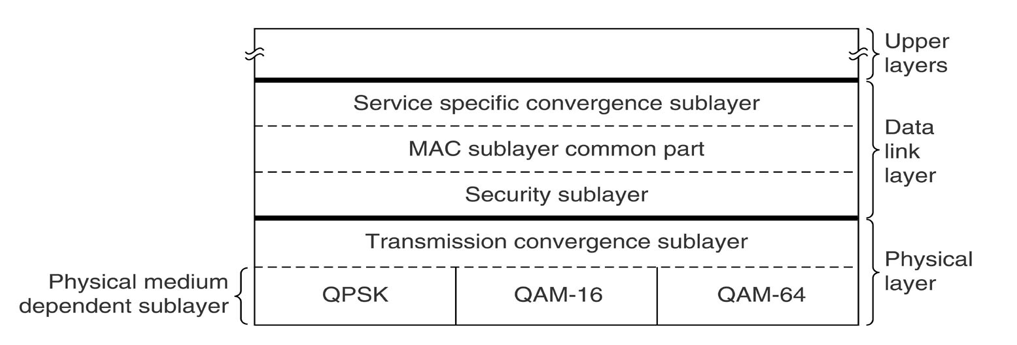
\includegraphics[scale=0.338]{chapters/3/assets/schema_z.png}
            \end{center}

        \subsubsection{Formato dei frame 802.16}
            I signficati dei campi dei frame sono i seguenti:
            \begin{itemize}
                \item \textbf{EC}: indica che il frame è cifrato.
                \item \textbf{Type}: indica il tipo del frame.
                \item \textbf{CL}: indica se esiste un CRC finale.
                \item \textbf{EK}: indica le chiavi di codifica utilizzate.
                \item \textbf{Length}: è la lunghezza complessiva del frame.
                \item \textbf{ConnID}: indica la connessione di appartenenza del frame.
                \item \textbf{Header CRC}: è il CRC solo per l'header.
                \item \textbf{Payload}: può essere cifrato con chiavi simmetrica CBC o 3DES scambiate con chiave pubblica RSA e X509.
                \item il CRC finale è opzionale (i frame errati non saranno comunque ritrasmessi).
            \end{itemize}

            \begin{center}
                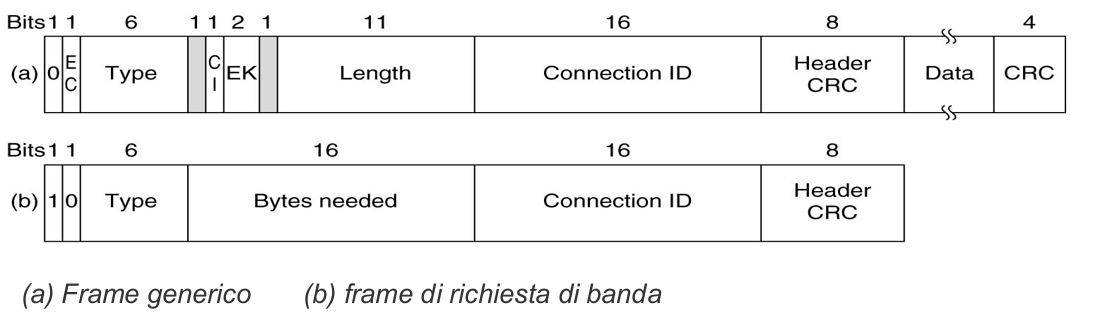
\includegraphics[scale=0.31]{chapters/3/assets/schema_za.png}
            \end{center}

    \subsection{Bluetooth}
        Nasce nel 1999 dall'associazione tra Sony-Ericsson, IBM, Toshiba e Nokia con l'obiettivo di realizzare un sistema di comunicazione senza fili tra dispositivi digitali e le loro periferiche.
        
        Sistema a bassa potenza, raggio 10 m, banda ISM a 2.4 GHz (no licenza).

        La banda è suddivisa in 79 canali di 1 MHz (1 bit per Hz, quindi al massimo 1Mb/s) e utilizza Frequency Hopping Spread Spectrum.
        
        Un dispositivo \textbf{Bluetooth Master} può gestire simultaneamente la comunicazione fino a 7 nodi slave entro un raggio di 10 metri, realizzando una \textbf{Piconet}.

        Due nodi Slave non possono comunicare tra loro.

        Due Piconet possono essere collegate tra loro mediante un nodo condiviso, formando una rete allargata denominata \textbf{ScatterNet}.
        
        802.15 è una emanazione di IEEE in cui è definita la WPAN (Wireless Personal Area Network), attualmente sono definiti solo lo strato fisico e data link.